\documentclass{article}
\usepackage{amsmath}
\usepackage{amssymb}
\usepackage{amsfonts}
\usepackage{mathtools}
\usepackage{mathrsfs}
\usepackage{amsthm}
\usepackage{bbm}
\usepackage{graphicx}
\usepackage{pgfplots}
\usepackage{tikz}

\title{Differential Equations - MATH246}
\author{Tom Mitchell}
\date{Conway -Fall 2024}

\begin{document}

\maketitle

\section*{Class Information}

\subsection*{Grading}
\begin{itemize}
    \item Matlab assignments — 18\% (6\% each)
    \item Quizzes (drop two lowest) — 17\%
    \item Two best in-class exams — 17\% each
    \item Worst in-class exam — 8\%
    \item Final exam — 23\%
\end{itemize}

\subsection*{Office Hours}
\begin{itemize}
    \item Monday: 2:00 PM - 3:00 PM (in person, Kirwin 2400)
    \item Tuesday: 1:15 PM - 2:30 PM (in person, Kirwin 2400)
    \item TBA: Zoom (online)
\end{itemize}

\subsection*{Exams}
\begin{itemize}
    \item 3 midterms and a final exam
\end{itemize}

\section*{Day 1, Tuesday 8/27/2024}

\section*{Course Overview: (Differential Equations)}

\section*{Chapter 0:}

A differential equation is an algebraic relation between functions, their derivatives, and independent variables.

\pagebreak

\textbf{Examples:}
\begin{itemize}
    \item \( \left(\frac{dx}{dt}\right)^2 + x \sin(t) = \cos(x) \) \hfill \textit{(Order = 1)}
    \item \( y'' + ty' + y = \cos(t) \) \hfill (Note: \(y' = \frac{dy}{dt})\)\textit{(Order = 2)}
    \item \( \frac{dy}{dt} \cdot \frac{dy}{ds} + y \frac{dz}{dt} = \sin(st) \) \hfill \textit{(Order = 1)}
\end{itemize}

\textbf{Order:} The order of a differential equation is the order of the highest derivative that appears.

\textbf{Notation:} For \( \frac{dy}{dx} \), we can write \( y' \) or \( \dot{y} \) (dot notation).

An ordinary differential equation (ODE) involves no partial derivatives, as opposed to a partial differential equation (PDE).

\textbf{Note:} This course only deals with ODEs.

\subsection*{Linearity of ODEs}

An ODE with function \( y \) and independent variable \( t \) is \textbf{linear} if it can be written as:

\[
a_n(t)y^{(n)} + a_{n-1}(t)y^{(n-1)} + \dots + a_1(t)y' + a_0(t)y = f(t)
\]

\textit{where \( y^{(n)} \) is the \( n \)th derivative of \( y \).}

\textbf{Examples:}
\begin{itemize}
    \item \( \left(\frac{dx}{dt}\right)^2 + x \sin(t) = \cos(x) \) \hfill \textit{(Not linear: \( \left(\frac{dx}{dt}\right)^2 \) and \( \cos(x) \))}
    \item \( y'' + ty' + y = \cos(t) \) \hfill \textit{(Linear)}
    \item \( y^{(4)} + y^{(2)} = 2 \) \hfill \textit{(Linear)}
\end{itemize}

\subsection*{Systems of ODEs}

A system of ODEs consists of multiple ordinary differential equations that are considered together:

\[
\left\{
\begin{array}{l}
\text{ODE} 1 \\
\text{ODE} 2 \\
\vdots \\
\text{ODE} n
\end{array}
\right.
\]

\section*{Chapter 1: Introduction}

\subsection*{Section 1: First-Order ODEs}

First-order ODEs can be complicated. We will focus on those that can be put into the standard form \(\boxed{\frac{dy}{dt} = f(t, y)}\).

\textbf{Example:} Consider the equation \(\frac{dw}{dz} = \frac{-z}{6w}\). This can be rewritten as:

\[
\frac{dw}{dz} = \frac{-z}{6w}
\]

A function \(Y(t)\) is a solution to \(y' = f(t, y)\) on the interval \((a, b)\) if:

\begin{itemize}
    \item \(Y(t)\) and \(Y'(t)\) exist on \((a, b)\),
    \item \(f(t, Y(t))\) exists on \((a, b)\), and
    \item \(Y'(t) = f(t, Y(t))\) on \((a, b)\).
\end{itemize}

\textbf{Example:} Consider the equation \(y'(t) = \frac{t}{y}\) with the solution \(Y(t) = \sqrt{4 - t^2}\).

To check this, calculate:

\[
Y'(t) = \frac{-t}{\sqrt{4 - t^2}}
\]

\(Y(t)\) is defined on the interval \([-2, 2]\), but \(f(t, Y(t)) = \frac{t}{\sqrt{4 - t^2}}\) is only defined for \((-2, 2)\), not at \(\pm 2\). Therefore, \(Y(t)\) is a solution on \((-2, 2)\), not on \([-2, 2]\).

\subsubsection*{Explicit Equations}

These are of the form \( y' = f(t) \).

The general solution is:

\[
y = \int f(t) \, dt = F(t) + C
\]

where \( F(t) \) is an antiderivative of \( f(t) \) (i.e., \( F'(t) = f(t) \)) and \( C \) is a constant.

\textbf{Example:} Consider the ODE

\[
\frac{dy}{dx} = 2x + 1
\]

The general solution is:

\[
y = x^2 + x + C
\]

\textbf{Graph for different values of \( C \):}

\begin{center}
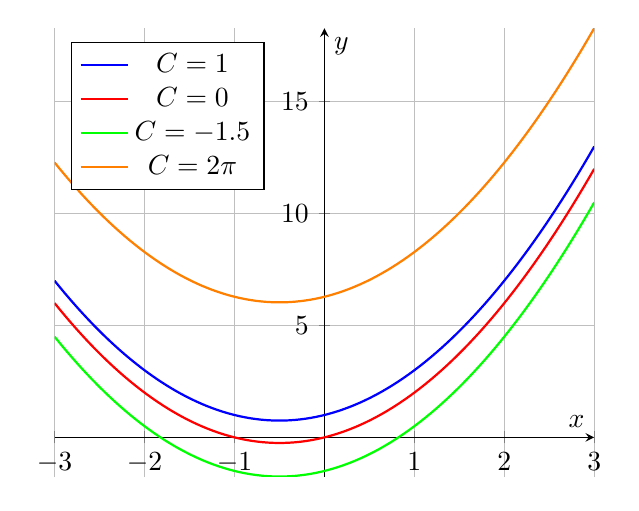
\begin{tikzpicture}
    \begin{axis}[
        xlabel={$x$},
        ylabel={$y$},
        axis lines=middle,
        grid=major,
        legend pos=north west,
        domain=-3:3,
        samples=100
    ]
    \addplot[blue, thick] {x^2 + x + 1};
    \addlegendentry{$C = 1$}
    
    \addplot[red, thick] {x^2 + x};
    \addlegendentry{$C = 0$}
    
    \addplot[green, thick] {x^2 + x - 1.5};
    \addlegendentry{$C = -1.5$}
    
    \addplot[orange, thick] {x^2 + x + 2*pi};
    \addlegendentry{$C = 2\pi$}
    \end{axis}
\end{tikzpicture}
\end{center}

To select a specific solution from the general solution, we need an initial condition: \( \boxed{y(t_I) = y_I} \).

The pair \( y' = f(t) \) with \( y(t_I) = y_I \) is called an Initial Value Problem (IVP).

\textbf{Example: Solve the IVP}

\[
\frac{dy}{dx} = 2x + 1 \quad \text{with} \quad y(0) = 2
\]

\textbf{Solution:}

Start with the general solution:

\[
y = x^2 + x + C
\]

Using the initial condition \( y(0) = 2 \):

\[
2 = 0^2 + 0 + C \quad \Rightarrow \quad C = 2
\]

Thus, the specific solution is:

\[
y = x^2 + x + 2
\]

\subsubsection*{Interval of Definition/Existence}

The interval of definition/existence of a solution to an IVP is the \textbf{largest} interval \( (a, b) \) where:

\begin{itemize}
    \item \( t_I \in (a, b) \)
    \item \( f(t) \) is continuous on \( (a, b) \)
\end{itemize}

\section*{Chapter 2: Linear Equations}

These look like:

\[
p(t) y' + q(t) y = r(t) \quad \text{where } p(t) \neq 0 \text{ for the values of } t \text{ we are considering.}
\]

In standard form:

\[
y' = -\frac{q(t)}{p(t)} y + \frac{r(t)}{p(t)}
\]

Let:

\[
a(t) = \frac{q(t)}{p(t)}, \quad f(t) = \frac{r(t)}{p(t)}
\]

We write it as:

\[
y' + a(t) y = f(t)
\]

Here, \( f(t) \) is called the forcing function.

If \( f(t) = 0 \), the ODE is called homogeneous; otherwise, it is non-homogeneous.

\subsection*{Recipe for Solving First-Order Linear ODEs}

Given:

\[
y' + a(t) y = f(t)
\]

1. Choose an antiderivative \( A(t) \) of \( a(t) \).
2. Multiply both sides by \( e^{A(t)} \):

\[
e^{A(t)} y' + a(t) e^{A(t)} y = f(t) e^{A(t)}
\]

Let:

\[
f(t) e^{A(t)} = g(t)
\]

This simplifies to:

\[
\frac{d}{dt} \left( e^{A(t)} y \right) = g(t)
\]

3. Integrate both sides:

\[
e^{A(t)} y = G(t) + C \quad \Rightarrow \quad y = e^{-A(t)} G(t) + C e^{-A(t)}
\]

This is the general solution.

\textbf{Example:} Solve the ODE

\[
\frac{dy}{dt} = -y
\]

1. Rewrite as \( y' + y = 0 \).
2. Here, \( a(t) = 1 \), so choose \( A(t) = t \).
3. Multiply both sides by \( e^t \):

\[
e^t y' + e^t y = 0 \quad \Rightarrow \quad \frac{d}{dt} (e^t y) = 0
\]

4. Integrate:

\[
e^t y = C \quad \Rightarrow \quad y = C e^{-t}
\]

This is the general solution.

\textbf{Example:} Consider the ODE

\[
y' = -y + e^t
\]

1. Rewrite as \( y' + y = e^t \).
2. Here, \( a(t) = 1 \), so choose \( A(t) = t \).
3. Multiply both sides by \( e^t \):

\[
e^t y' + e^t y = e^{2t} \quad \Rightarrow \quad \frac{d}{dt} (e^t y) = e^{2t}
\]

4. Integrate:

\[
e^t y = \frac{1}{2} e^{2t} + C \quad \Rightarrow \quad y = \frac{1}{2} e^t + C e^{-t}
\]

This is the general solution.

\textbf{Example: Solve the IVP}

\[
\frac{dx}{dt} + \cos(t)x = \cos(t) \quad \text{with} \quad x\left(\frac{\pi}{2}\right) = 0
\]

\textbf{Solution:}

1. Here, \( a(t) = \cos(t) \), so choose \( A(t) = \sin(t) \).
2. Multiply both sides by \( e^{\sin(t)} \):

\[
e^{\sin(t)} x' + \cos(t) e^{\sin(t)} x = \cos(t) e^{\sin(t)}
\]

This simplifies to:

\[
\frac{d}{dt} \left( e^{\sin(t)} x \right) = \cos(t) e^{\sin(t)}
\]

3. Integrate:

\[
e^{\sin(t)} x = \int \cos(t) e^{\sin(t)} \, dt = e^{\sin(t)} + C
\]

Thus,

\[
x = 1 + C e^{-\sin(t)}
\]

4. Apply the initial condition \( x\left(\frac{\pi}{2}\right) = 0 \):

\[
0 = 1 + C e^{-1} \quad \Rightarrow \quad C = -e
\]

Thus, the specific solution is:

\[
x = 1 - e^{1 - \sin(t)}
\]

\section*{Day 2, 8/27/2024}

I.2 (continued)

\section*{Problem Statement}

Consider the initial value problem (IVP):

\[
y' + a(t)y = f(t), \quad y(t_I) = y_I
\]

\textbf{Theorem:}  
If \( a(t) \) and \( f(t) \) are continuous over the interval \( (a, b) \) and \( t_I \in (a, b) \), then there is a unique solution to the IVP that is continuous on \( (a, b) \), and it's given by our method.

\section*{Example}

Consider the differential equation:

\[
z' + \cot(t)z = \frac{1}{\ln(t^2)}, \quad z(4) = 3
\]

Find the largest interval on which we can guarantee a unique continuous solution to this IVP.

\section*{Solution}

The function \( \ln(t^2) \) is continuous on \( (-\infty, 0) \) and \( (0, \infty) \), but \( \frac{1}{\ln(t^2)} \) is discontinuous at \( t = 0 \) and when \( \ln(t^2) = 0 \), i.e., \( t = \pm 1 \).

The function \( \cot(t) \) has discontinuities at multiples of \( \pi \).

The largest interval of continuity that includes \( t = 4 \) is \( (\pi, 2\pi) \).


\begin{center}
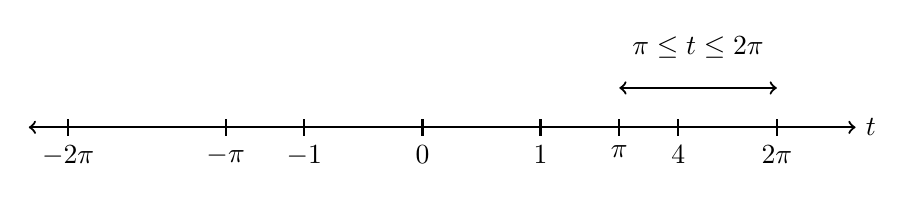
\begin{tikzpicture}

% Draw the line
\draw[thick, <->] (-5,0) -- (5.5,0) node[right] {$t$};

% Mark and label specific points
\foreach \x/\xtext in {-4.5/$-2\pi$, -2.5/$-\pi$, -1.5/$-1$, 0/$0$, 1.5/$1$, 2.5/$\pi$, 4.5/$2\pi$}
  \draw[thick] (\x,3pt) -- (\x,-3pt) node[below] {\xtext};

% Mark the point 4
\draw[thick] (3.25,3pt) -- (3.25,-3pt) node[below] {$4$};

% Draw the interval of continuity
\draw[thick,<->] (2.5,0.5) -- (4.5,0.5);
\node at (3.5,0.75) [above] {$\pi \leq t \leq 2\pi$};

\end{tikzpicture}
\end{center}


\section*{I.3: Separable Equation}

A first-order ordinary differential equation (ODE) is \textbf{separable} if it can be written in the form:

\[
y' = f(t)g(y)
\]

\textbf{Example:}

Consider the differential equation:

\[
y' = 2ty^2 + 3t^2y^2
\]

We can factor this as:

\[
y' = (2t + 3t^2)y^2
\]

Here, we have:

\[
f(t) = 2t + 3t^2, \quad g(y) = y^2
\]

An ODE of the form \( y' = g(y) \) is called \textbf{autonomous}.

A solution is called \textbf{stationary} if it is constant. If \( y = C \) is a stationary solution, then:

\[
y' = 0 \Rightarrow \boxed{0 = g(C)}
\]

\textbf{Example:}

Consider the equation:

\[
y' = 4y - y^3
\]

To find the stationary solutions, set:

\[
4y - y^3 = 0 \Rightarrow y(4 - y^2) = 0 \Rightarrow y(2 - y)(2 + y) = 0
\]

Thus, the stationary solutions are:

\[
y = 0, \quad y = 2, \quad y = -2
\]




\section*{Non-Stationary Solutions}

To find non-stationary solutions of the equation \( y' = g(y) \), we proceed as follows:

\[
y' = g(y) \quad \Rightarrow \quad \frac{1}{g(y)} y' = 1 
\]

Taking the integral on both sides:

\[
\int \frac{1}{g(y)} y' \, dt = \int 1 \, dt
\]

This simplifies to:

\[
\int \frac{1}{g(y)} \, dy = t + C
\]

The result is an implicit equation for our solution.

\textbf{Why can we divide by \( g(y) \)?}  
\( g(y) = 0 \) corresponds to stationary solutions, and we are looking for non-stationary solutions, i.e., \( g(y) \neq 0 \).

\section*{Example: Find All Solutions to \( y' = y^2 \)}

\textbf{Stationary Solutions:}  
Set \( y^2 = 0 \), which implies \( y = 0 \).

\textbf{Non-Stationary Solutions:}

Starting with the equation:

\[
\frac{1}{y^2} y' = 1
\]

Integrate both sides:

\[
\int \frac{1}{y^2} y' \, dt = \int 1 \, dt
\]

This simplifies to:

\[
\int \frac{1}{y^2} \, dy = t + C
\]

Evaluating the integral:

\[
-\frac{1}{y} = t + C
\]

We can find an explicit solution:

\[
-y = \frac{1}{t + C} \quad \Rightarrow \quad y = -\frac{1}{t + C}
\]



Each solution \( y = -\frac{1}{t + C} \) actually represents two solutions, one defined on \( (-\infty, -C) \) and the other on \( (-C, \infty) \).

\textbf{Note:} Our solution is discontinuous even though all functions in the original equation \( y' = y^2 \) are continuous.

\section*{General Separable Equations}

Consider the general separable equation:

\[
y' = f(t)g(y)
\]

If \( g(c) = 0 \), then \( y = c \) is a stationary solution (so set g(y) = 0).

For non-stationary solutions:

\[
\frac{1}{g(y)} y' = f(t)
\]

Taking the integral on both sides:

\[
\int \frac{1}{g(y)} y' \, dt = \int f(t) \, dt
\]

This simplifies to:

\[
\int \frac{1}{g(y)} \, dy = F(t) + C
\]

\section*{Example: Find All Solutions to \( \frac{dz}{dx} = \frac{3x + xz^2}{z + x^2z} \)}

First, rewrite the equation:

\[
\frac{dz}{dx} = \frac{x}{1 + x^2} \cdot \frac{3 + z^2}{z}
\]

Thus, we identify:

\[
f(x) = \frac{x}{1 + x^2}, \quad g(z) = \frac{3 + z^2}{z}
\]

\textbf{Stationary Solutions:}  
Set \( g(z) = 0 \):

\[
\frac{3 + z^2}{z} = 0 \quad \Rightarrow \quad 3 + z^2 = 0
\]

This equation has no real solution, so there are no stationary solutions.

\textbf{Non-Stationary Solutions:}

Start with:

\[
\frac{1}{g(z)} \frac{dz}{dx} = f(x)
\]

Which simplifies to:

\[
\frac{z}{3 + z^2} \cdot \frac{dz}{dx} = \frac{x}{1 + x^2}
\]

Integrate both sides:

\[
\int \frac{z}{3 + z^2} \frac{dz}{dx} \, dx = \int \frac{x}{1 + x^2} \, dx
\]

Use substitution:

- Let \( u = 3 + z^2 \), then \( du = 2z \, dz \).
- Let \( v = 1 + x^2 \), then \( dv = 2x \, dx \).

The integrals become:

\[
\int \frac{1}{2u} du = \int \frac{1}{2v} dv
\]

This integrates to:

\[
\frac{1}{2} \ln|u| = \frac{1}{2} \ln|v| + C
\]

Substituting back \( u \) and \( v \):

\[
\frac{1}{2} \ln|3 + z^2| = \frac{1}{2} \ln|1 + x^2| + C
\]



\section*{Initial Value Problems (IVPs)}

\textbf{Example:} Solve the initial value problem:

\[
y' = ty^2 - ty, \quad y(1) = 2
\]

We can factor the equation as:

\[
y' = t(y^2 - y)
\]

\textbf{Stationary Solutions:}  
Set \( y^2 - y = 0 \):

\[
y(y - 1) = 0 \quad \Rightarrow \quad y = 0 \quad \text{or} \quad y = 1
\]

Neither \( y = 0 \) nor \( y = 1 \) satisfies the initial condition \( y(1) = 2 \).

\begin{center}
\begin{tikzpicture}
    \draw[thick,->] (-1,0) -- (3,0) node[right] {$t$};
    \draw[thick,->] (0,-1) -- (0,3) node[above] {$y$};
    
    \draw[blue,thick] (-1,1) -- (3,1) node[below right] {$y=1$};
    \draw[red,thick] (-1,0) -- (3,0) node[below right] {$y=0$};

    \node at (1,2) [circle,fill,inner sep=1.5pt,label=above:{$(1,2)$}] {};
\end{tikzpicture}
\end{center}

As shown in the graph, neither \( y = 0 \) nor \( y = 1 \) passes through the point \( (1, 2) \).

\textbf{Other Solutions:}  
We solve the differential equation for non-stationary solutions:

\[
\frac{1}{y^2 - y} \frac{dy}{dt} = t \quad \Rightarrow \quad \frac{1}{y^2 - y} \, dy = t \, dt
\]

Integrate both sides:

\[
\int \frac{1}{y^2 - y} \, dy = \int t \, dt
\]

Using partial fractions:

\[
\frac{1}{y(y-1)} = \frac{A}{y} + \frac{B}{y-1}
\]

This leads to:

\[
1 = A(y - 1) + B(y) 
\]

By guessing \( A = -1 \) and \( B = 1 \), we get:

\[
\int \left( -\frac{1}{y} + \frac{1}{y-1} \right) dy = \int t \, dt
\]

Integrating both sides:

\[
-\ln|y| + \ln|y - 1| = \frac{t^2}{2} + C
\]

Using the logarithm property \( \ln(a) - \ln(b) = \ln\left(\frac{a}{b}\right) \), this simplifies to:

\[
\ln\left|\frac{y - 1}{y}\right| = \frac{t^2}{2} + C
\]

\textbf{Applying the Initial Condition:}  
Given \( y(1) = 2 \):

\[
\ln\left|\frac{2 - 1}{2}\right| = \frac{1^2}{2} + C
\]

\[
\ln\left(\frac{1}{2}\right) = \frac{1}{2} + C \quad \Rightarrow \quad C = \ln\left(\frac{1}{2}\right) - \frac{1}{2}
\]

Substituting \( C \) back into the equation:

\[
\ln\left|\frac{y - 1}{y}\right| = \frac{t^2}{2} + \ln\left(\frac{1}{2}\right) - \frac{1}{2}
\]




\section*{Uniqueness and Existence Theorem}

If \( f(t) \) is continuous on \( (a, b) \) and \( g(y) \) is continuous and differentiable on \( (c, d) \), then for every \( t_I \in (a, b) \) and \( y_I \in (c, d) \), there exists a unique continuous solution to the equation

\[
y' = f(t)g(y)
\]

with the initial condition \( y(t_I) = y_I \), defined on some interval around \( t_I \). The solution is determined by our method.

\section*{Example}

Consider the differential equation:

\[
\frac{dy}{dt} = 3y^{2/3}, \quad y(0) = 0
\]

\textbf{Stationary Solution:}  
\( y = 0 \) is a stationary solution, and it solves our initial value problem (IVP).

However, \( g(y) = 3y^{2/3} \) is not differentiable at \( y = 0 \), so we might have other solutions.

\textbf{Finding Other Solutions:}

\[
\frac{1}{3y^{2/3}} \frac{dy}{dt} = 1
\]

Integrating both sides:

\[
\int \frac{1}{3y^{2/3}} \, dy = \int 1 \, dt
\]

This simplifies to:

\[
y^{1/3} = t + C
\]

Raising both sides to the power of 3:

\[
y = (t + C)^3
\]

\textbf{Applying the Initial Condition:}  
For \( y(0) = 0 \), we get \( C = 0 \), so:

\[
y = t^3
\]

Thus, \( y = t^3 \) also solves our IVP.



















\end{document}
